\Chapter{Mérések, összehasonlítások}


\Section{Állandó idejű részek}
A program bizonyos részeinek sebessége nem, vagy csak minimálisan függ az adatok mennyiségétől. Vizsgáljuk először ezeket a részeket.

Kernelkód beolvasása a fájlból.
40 mikroszekundum.

Kapcsolat létrehozása az adatbázis szerverrel:
16500 mikroszekundum.

OpenCL: driver kontextus, parancssor
50 000 mikroszekundum

Program létrehozása és felépítése az eszközhöz
1000 mikroszekundum

\Section{Adatmennyiségtől függő részek}

Adatok mozgatása.
A legjelentősebb rész hatékonyság szempontjából az adatok mozgatási sebessége.
\SubSection{A MySQL Connector sebessége}
Ezt a sebességet legpontosabban úgy kaphatjuk meg ha a program következő két sorának idejét vizsgáljuk.
\begin{python}
pstmt = con->prepareStatement(command);
res = pstmt->executeQuery();
\end{python}
Ahhol \texttt{command} egy \texttt{String} az SQL parancs és a következő módon áll össze:
\begin{python}
range=32768;
    while(i <= 1048576){
    		command = "SELECT * FROM speedtest_1048576 Limit " 
    			+ to_string(i);
    		. . .
   	 	i+=range;
    }
\end{python}
Ezen kívül a a grafikonon látható tüskék mértékének csökkentése érdekében minden lekérdezést 5x futtattam és idejüket átlagoltam.
\begin{itemize}
\item A LIMIT hozzáadása a lekérdezéshez nem növeli annak idejét.
\item A tábla tartalmaz elsődleges kulcsot. Amennyiben nincs a lekérdezés ideje nő.
\item A lekérdendő oszlopokat manuálisan módosítottam a programban. 
\begin{itemize} 
\item \texttt{SELECT c1p1 FROM ...}
\item \texttt{SELECT c1p1, c2 FROM ...} 
\item \texttt{SELECT c1p1, c2, c3 FROM ...} 
\item \texttt{SELECT * FROM ...} 
\end{itemize}
\end{itemize}

\begin{figure}[h!]
\centering
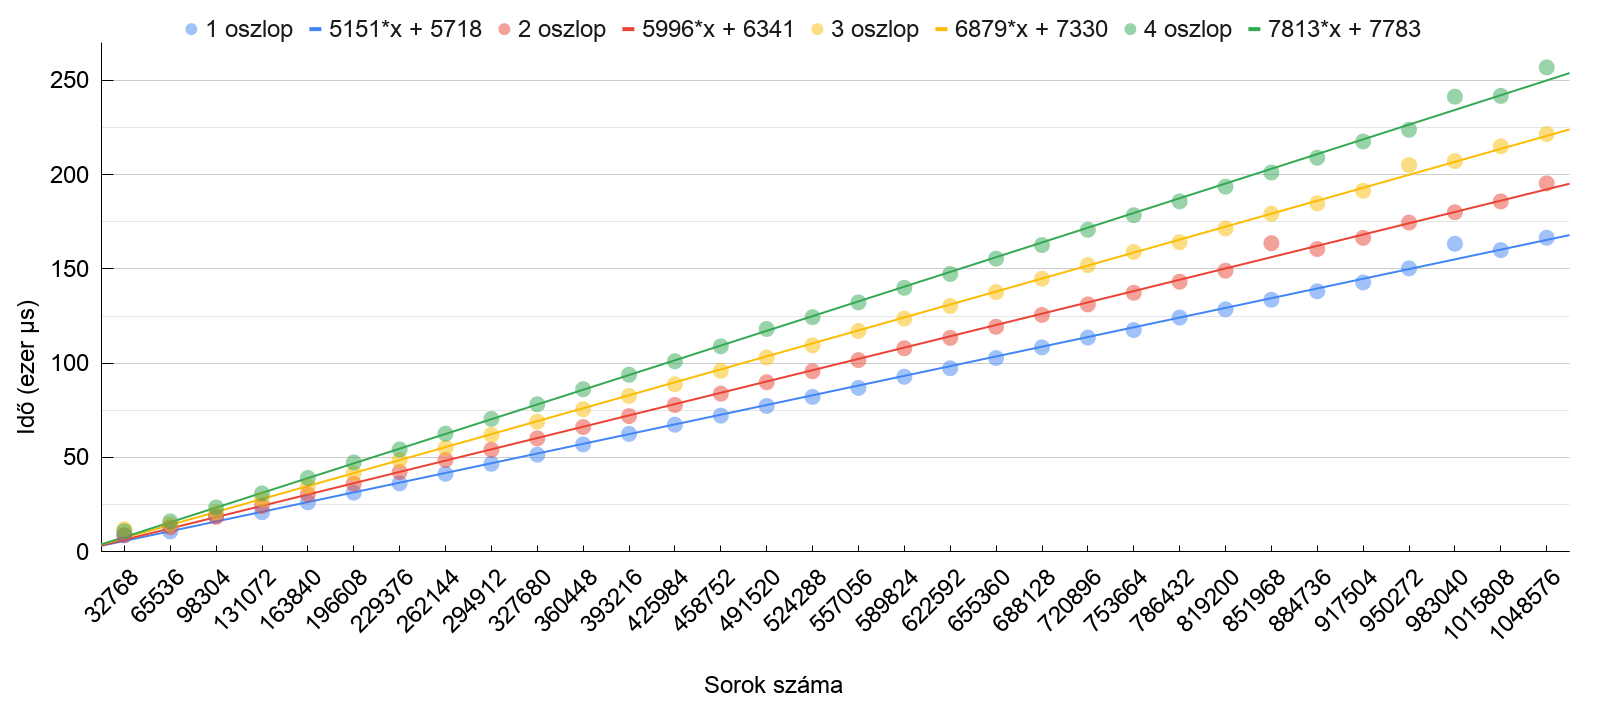
\includegraphics[width=\textwidth]{images/sqlquery.png}
\caption{SQL lekérdezési sebessége}
\label{fig:schema}
\end{figure}
%BETŰMÉRET NAGYÍTÁSRA SZORUL
Az ábrán, egyértelműen látható, hogy a sorok számának növekedésével az idő is lineárisan nő.
Jelmagyarázatnál látható egyenes egyenletekből becsléseket lehet készíteni adott sorszámhoz. Négy oszlop felett a 4 oszlop idejét kell használni megfelelő szorzóval.

4 és 6 oszlop esetén:
$$ x = \text{sorok száma}/32768 - 1 $$
$$ 7813 * \text{sorok száma} + 7783 = \text{lekérdezés ideje}$$
$$ \text{lekérdezés ideje} * 1.5 = \text{lekérdezés ideje 6 oszlopra} $$


\SubSection{A query válaszának átmásolása a struktúra tömbbe}
A másik hatékonyságot rendkívül romboló rész, amikor az adatokat átmásoljuk a saját tömbünkbe.
A mért program szakasz:

\begin{python}
int i = 0;
*T1_size = res->rowsCount();
*T1 = (Table1Type*) malloc(sizeof(Table1Type) * *T1_size);

while (res->next())
	{
		T1[0][i].c1p1 = res->getInt("c1p1");
		T1[0][i].c2 = res->getInt("c2");
		T1[0][i].c3 = res->getInt("c3");
		T1[0][i].c4 = res->getInt("c4");
		i++;
	}
delete res;
delete pstmt;
\end{python}

Itt a válaszból lekérdezzük a méretet, majd ez alapján létrehozzuk a saját objektumunkat a memóriában, ezután egyesével belemásoljuk 
a kapott adatokat soronként.
Az mérési módszer megegyezik az előzőekben használtakkal.
A texttt{res} és texttt{pstmt} törlése időméréskor nagyon fontos, ugyanis ennek kihagyása miatt a memória megtelhet!


\begin{figure}[h!]
\centering
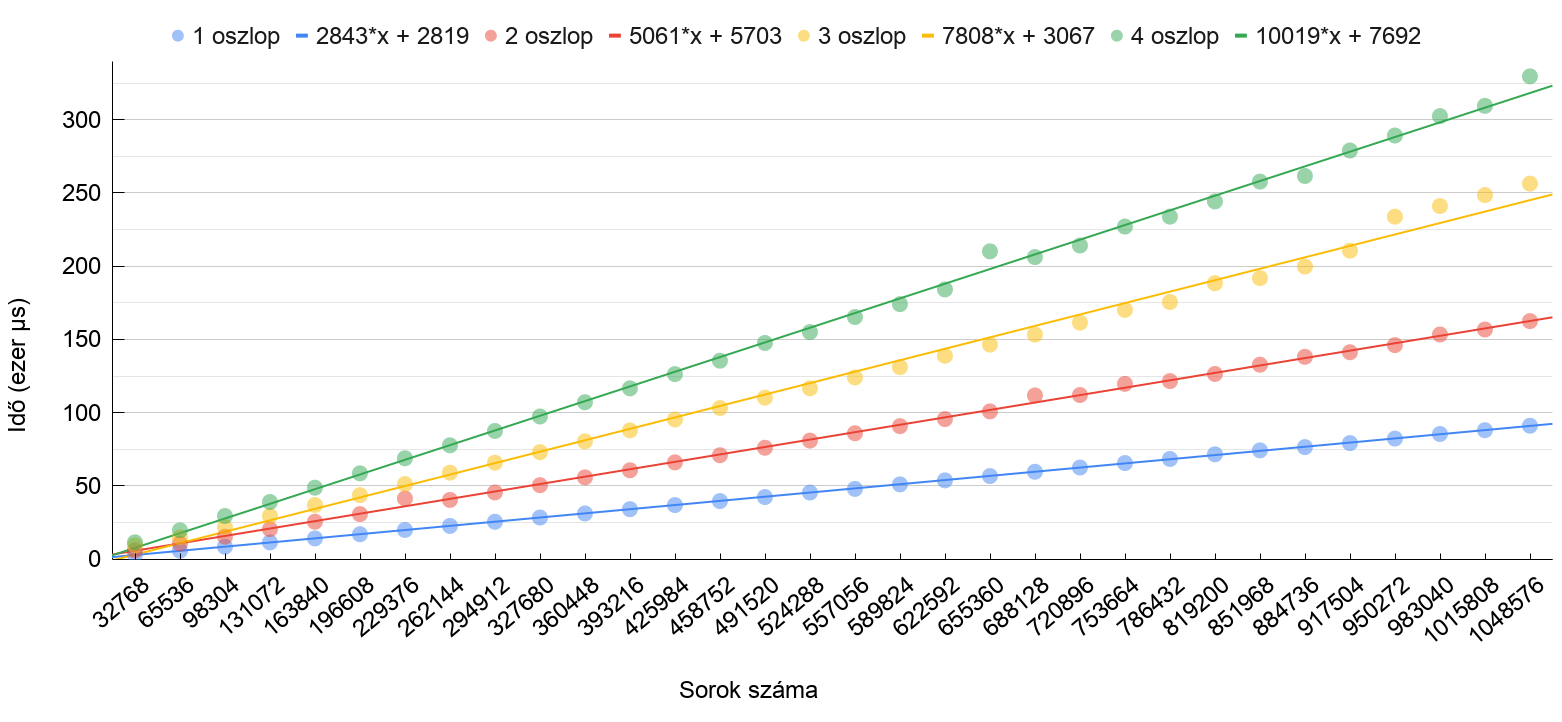
\includegraphics[width=\textwidth]{images/ccopy.png}
\caption{Adatok másolása saját tömbbe}
\label{fig:schema}
\end{figure}

A grafikonon két dolgot vehetünk észre azonnal. Az egyik az, hogy ez a folyamat lassabb mint maga a lekérdezés a másik pedig, hogy drasztikusabb a növekedés az oszlopok számának sokasodásával.
Tegyük fel, hogy 4 oszlop felett már nincs szignifikáns eltérés az időnövekedésben. Ekkor használhatjuk az előbb is használt módszert a becslésekhez.

Másolás becslése 4 és 6 oszlop esetén:
$$ x = \text{sorok száma}/32768 - 1 $$
$$ 10019 * x + 7692 = \text{másolás ideje}$$
$$ \text{másolás ideje} * 1.5 = \text{másolás ideje 6 oszlopra} $$

\SubSection{Adatok bemásolása a pufferekbe}

Az adatok átmásolása az OpenCL puffereibe szintén egy olyan része a programnak, ami sok időt emészthet fel.
Vizsgált rész:

\begin{python}
int range=65536;
while( range <= 1048576){
 clStatus = clEnqueueWriteBuffer(command_queue, Table1_clmem,
  CL_TRUE, 0, range * sizeof(Table1Type), t1, 0, NULL, NULL);
 clStatus = clEnqueueWriteBuffer(command_queue, Table_size_clmem,
  CL_TRUE, 0, sizeof(int), &t1_size, 0, NULL, NULL);
 clStatus = clEnqueueWriteBuffer(command_queue, Interval_size_clmem,
  CL_TRUE, 0, sizeof(int), &interval_size, 0, NULL, NULL);
 clStatus = clFinish(command_queue);
	range += 65536;
}
\end{python}

A mérés a belső 4 sorra vonatkozik. 

\begin{figure}[h!]
\centering
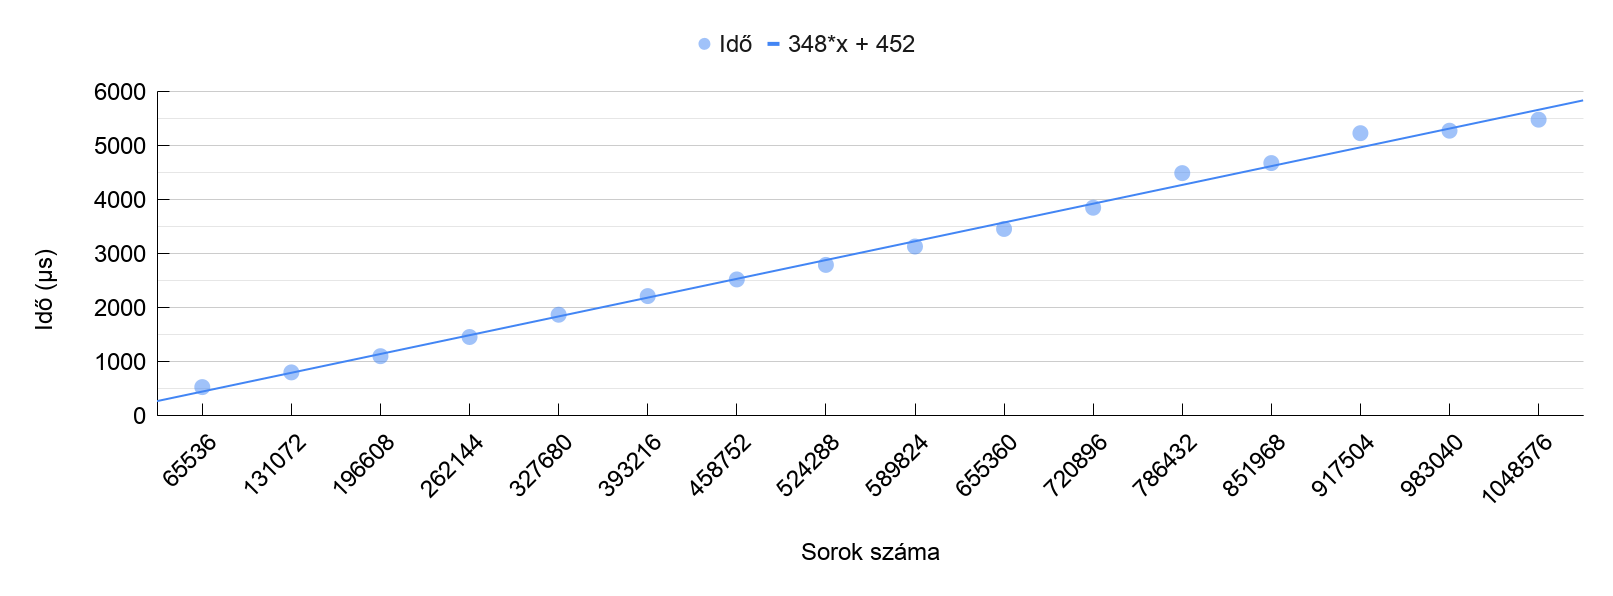
\includegraphics[width=\textwidth]{images/inpuffer.png}
\caption{Adatok kimásolása 2.}
\label{fig:schema}
\end{figure}

Mivel ebben az esetben a másolás egybefüggő memória területre vonatkozik, nem pedig elemenkénti hivatkozás, ezért elegendő egyetlen mérés.
A grafikonon egy 4 oszlopos tábla átmásolásának a sebessége látható. Ebből Több vagy kevesebb oszlopra a becslés egyszerű szorzásokkal megkapható.

4 és 3 oszlop esetén:
$$ x = \text{sorok száma} / 65536 $$
$$ 348*x + 452 = \text{pufferbe másolás ideje} $$ 
$$ \text{pufferbe másolás ideje} * 0.75 = \text{3 oszlopos pufferbe másolás ideje}  $$



\SubSection{Adatok kimásolása a pufferekből}

A program ezen részének hatékonysága már egy komplexebb vizsgálatot igényel.
Nézzük az első kiolvasási módszert, amikor a teljes válasz listát illetve a hozzá tartozó számlálót másoljuk ki.
Jelen mérésnél a lista csak egyetlen indexet tartalmaz. 

\begin{figure}[h!]
\centering
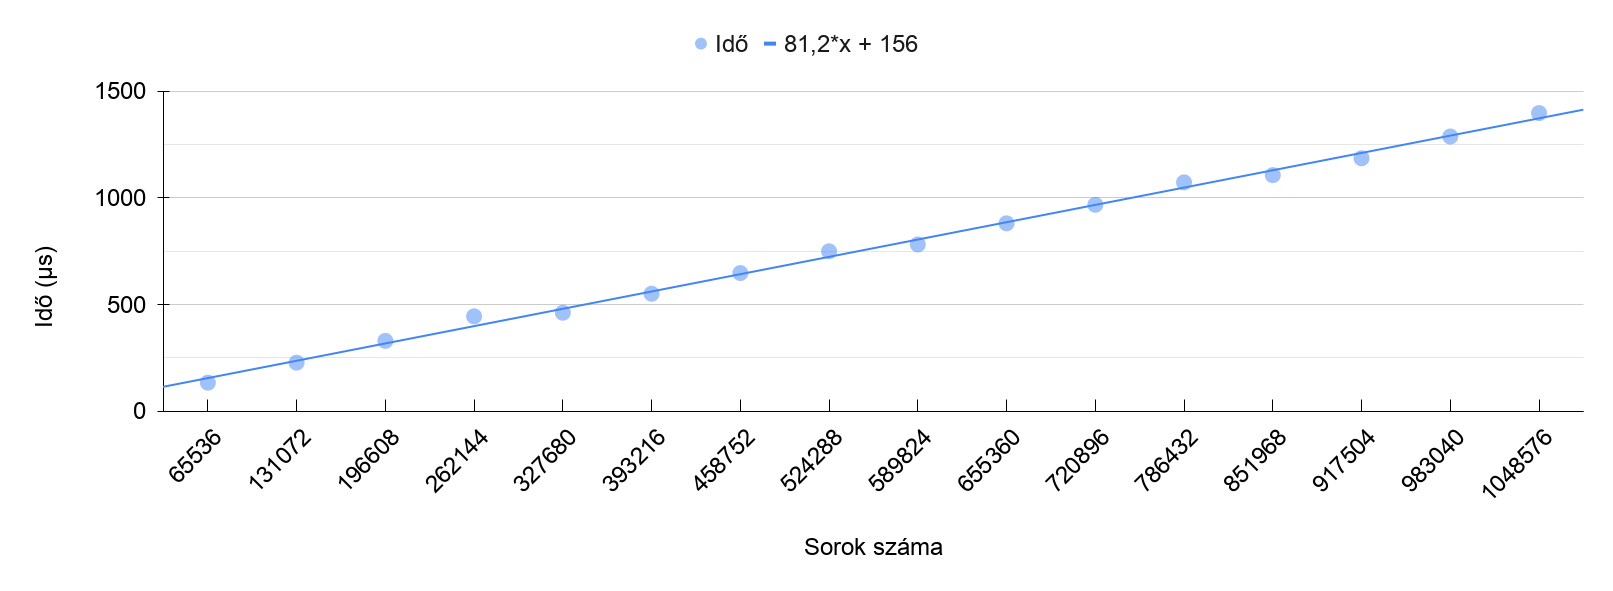
\includegraphics[width=\textwidth]{images/outpuffer.png}
\caption{Adatok kimásolása 2.}
\label{fig:schema}
\end{figure}

$$ 81,2*x + 156 = \text{puffer kiolvasási ideje} $$ 
Az előzőhöz hasonlóan itt is egy memória darabot másolunk, ennek szorzásával megkapjuk mennyi időbe telne a kiolvasás indexpárok vagy számított értékek hozzáadása esetén.
Ne felejtsük el, hogy ehhez tartozik egy számláló, ami jelen esetben a képlethez képest az elemszám gyöke, de két érték esetén már csak a felének a gyöke.
Ez azt jelenti, hogy $2^{20}$ -on érték esetén is a kiolvasási ideje csak megközelítőleg 37$\mu\text{s}$


A másik módszer miszerint nem olvassuk ki azonnal a választ, hanem alkalmazzuk az előző fejezetben taglalt optimalizálási eljárást.
Ennek hatékonysága a sok kisebb olvasás miatt függ az eredmények számától. Ennek méréséhez módosítani kell a kernel kódot, ezért maunálisan végeztem a méréseket, vagyis a szűrési feltételeket úgy módosítottam, hogy a találatok száma megfelelően változzon.
Fontos figyelembe venni, hogy a számok véletlenszerűek a táblázatban.

\begin{figure}[h!]
\centering
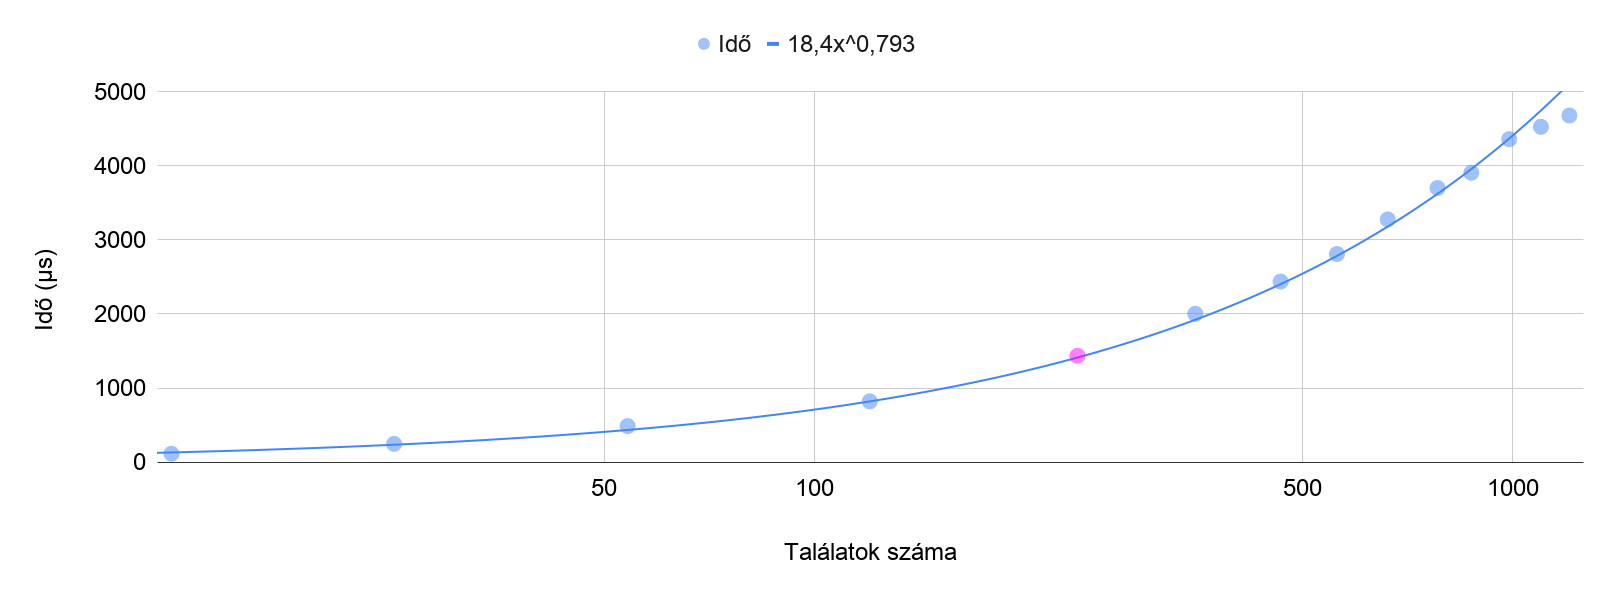
\includegraphics[width=\textwidth]{images/outpuffer2.png}
\caption{Adatok kimásolása 2.}
\label{fig:schema}
\end{figure}

Végeredményként látjuk, hogy ez a fajta kiolvasás rendkívül hatékony, de csak abban az esetben, ha a találatok száma minimális.
238 találatnál a módszer elérte azt az időt, ami alatt el lehet végezni a teljes másolást egy darabban.
\begin{figure}[h!]
\centering
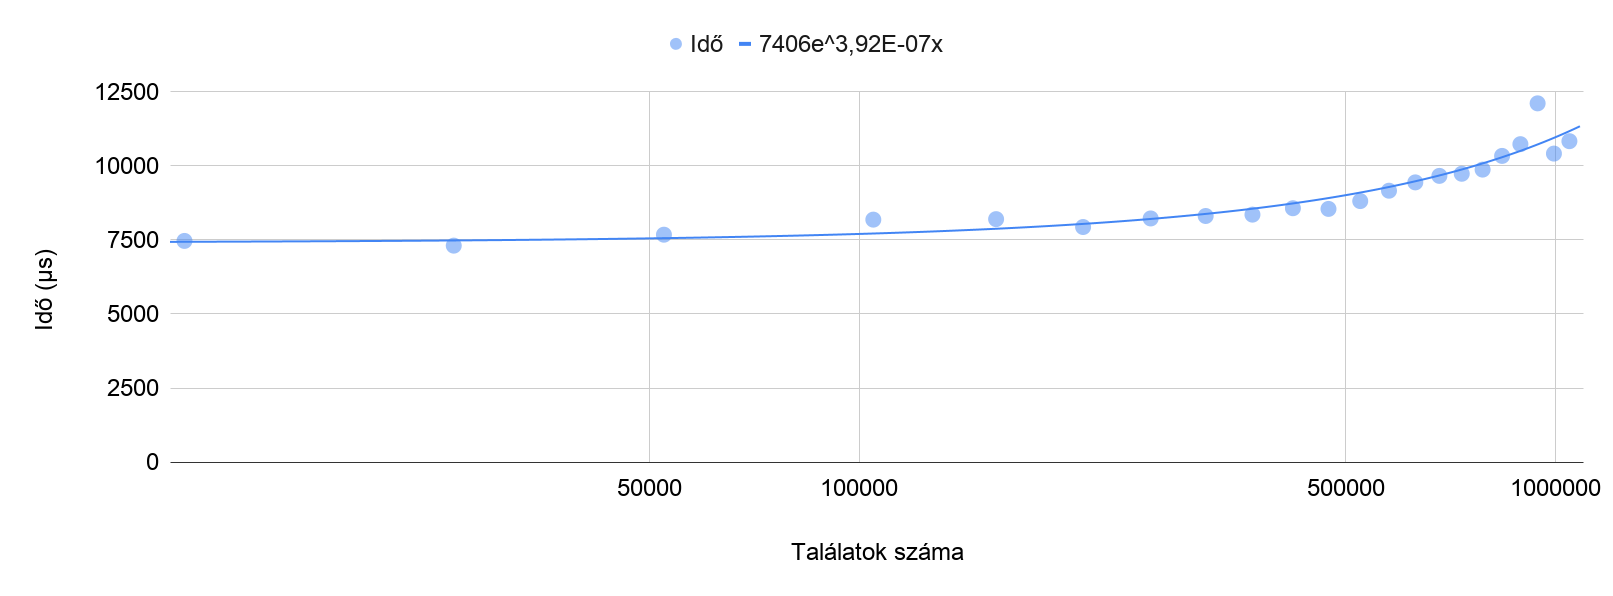
\includegraphics[width=\textwidth]{images/outpuffer3.png}
\caption{Adatok kimásolása 2.}
\label{fig:schema}
\end{figure}

\SubSection{A kernel sebessége}

\Section{Komplex lekérdezés hatékonysága}